% !TeX root = ../main.tex

\chapter{Modelos del transmisor y receptor}
\label{cap:transceptor}

\section{Introducci\'on}
\label{sec:trx-intro}

En este cap\'itulo se modelan el transmisor y el receptor. La
\cref{fig:cadena-bloques} muestra el esquema general de la cadena \'optica,
con los dos bloques marcados en rojo. El recuadro punteado es el enlace
\'optico del \cref{cap:canal}. El bloque de DSP es el objeto del
\cref{cap:dsp}.

\begin{figure}[H]
  \centering
  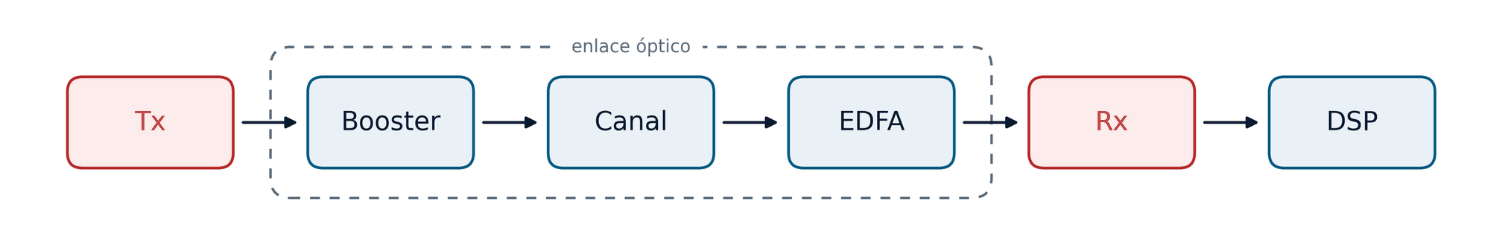
\includegraphics[width=0.95\linewidth]{CadenaOpticaBloques}
  \caption[Cadena completa de simulaci\'on]{%
    Cadena completa de simulaci\'on. En rojo, el transmisor y el receptor, que
    son los bloques que describe este cap\'itulo. Dentro del recuadro
    punteado, el enlace \'optico desarrollado en el \cref{cap:canal}. El DSP
    se trata en el \cref{cap:dsp}.}
  \label{fig:cadena-bloques}
\end{figure}

La \cref{tab:parametros} muestra los par\'ametros principales del transmisor y
del receptor. La elecci\'on de estos par\'ametros se hizo en base a valores de
dispositivos comerciales est\'andar y a los disponibles en el laboratorio, lo
que permite comparar la simulaci\'on con la medici\'on sobre la misma base en
el \cref{cap:experimental}.

\begin{table}[htbp]
\centering

\begin{tabular}{llc}
\toprule
\textbf{Par\'ametro} & \textbf{S\'imbolo} & \textbf{Valor} \\
\midrule
Tasa de s\'imbolo            & $\Rs$              & \SI{32}{\giga\baud} \\
Muestras por s\'imbolo       & SpS                & 16 (sim.) / 2 (DSP) \\
Polarizaciones               & $N_{\mathrm{pol}}$ & 2 \\
Roll-off del RRC             & $\beta$            & 0,2 \\
Longitud de onda             & $\lambda$          & \SI{1550}{\nano\metre} \\
Ancho de l\'inea por l\'aser & $\dnu$             & \SI{100}{\kilo\hertz} \\
Ancho de banda del Front end       & $B_{\mathrm{Rx}}$ & \SI{20}{\giga\hertz} \\
Ancho de banda del ADC       & $B_{\mathrm{ADC}}$ & \SI{33}{\giga\hertz} \\
\bottomrule
\end{tabular}
\caption[Par\'ametros principales de la simulaci\'on]{Par\'ametros principales de la simulaci\'on.}
\label{tab:parametros}
\end{table}

\section{Transmisor}
\label{sec:trx-tx}

\subsection{Generaci\'on de s\'imbolos y conformaci\'on de pulso}
\label{sec:trx-simbolos}

La secuencia de bits a transmitir se mapea en s\'imbolos QPSK con
codificaci\'on Gray, de forma independiente en cada polarizaci\'on. En las
simulaciones de este trabajo se emple\'o una secuencia pseudoaleatoria
PRBS-15, de longitud $2^{15}-1 = \num{32767}$, que es la misma que carga el
generador de patrones del laboratorio.

Los s\'imbolos generados se sobremuestrean a 16 muestras por s\'imbolo para
asegurar una tasa de muestreo de simulaci\'on suficientemente grande como para
representar la se\~nal \'optica sin aliasing. Despu\'es se conforman con un
filtro de ra\'iz de coseno alzado (RRC) de \emph{roll-off} $\beta = 0{,}2$. El
receptor luego incluye un segundo filtro RRC, el filtro adaptado, implementado
tambi\'en en el dominio digital. Entre los dos cumplen el criterio de Nyquist
y anulan la interferencia entre s\'imbolos en el instante de muestreo.

\begin{figure}[H]
  \centering
  \begin{subfigure}[b]{0.48\linewidth}
    \centering
    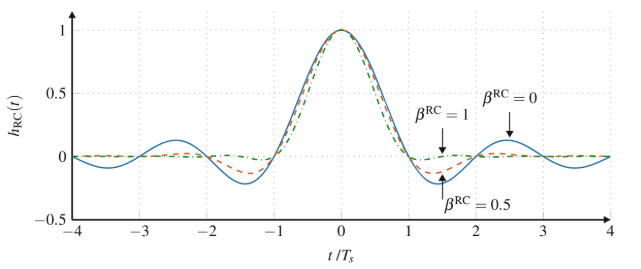
\includegraphics[width=\linewidth]{RRCtiempoLibro}
    \caption{}
  \end{subfigure}
  \hfill
  \begin{subfigure}[b]{0.48\linewidth}
    \centering
    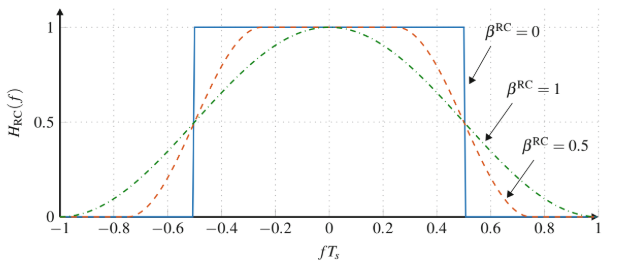
\includegraphics[width=\linewidth]{RRCfrecuenciaLibro}
    \caption{}
  \end{subfigure}
  \caption[Filtro de ra\'iz de coseno elevado]{%
    Filtro de ra\'iz de coseno elevado en tiempo~(a) y en frecuencia~(b) para
    distintos valores de \emph{roll-off}. Adaptado de~\cite{mello2021}.}
  \label{fig:rrc}
\end{figure}

La elecci\'on de $\beta$ presenta una relaci\'on de compromiso, y la
\cref{fig:rrc} lo muestra en los dos dominios. Un \emph{roll-off} chico
angosta el espectro, pero alarga las colas del pulso en el tiempo y lo vuelve
m\'as sensible al error de sincronismo, mientras que un \emph{roll-off} grande
hace lo contrario. A \SI{32}{\giga\baud} con $\beta = 0{,}2$, el ancho de
banda unilateral resulta
\begin{equation}
  B = \frac{\Rs\,(1+\beta)}{2} = \SI{19.2}{\giga\hertz}.
  \label{eq:ancho-senal}
\end{equation}
Con este valor la se\~nal entra justo en los \SI{20}{\giga\hertz} de ancho de
banda del Front end disponible, como se ver\'a en la \cref{sec:trx-rx}. A esto se suma que utilizar valores demasiado peque\~nos de $\beta$ degrada el
detector de error de tiempo de Gardner que se usa en el
\cref{cap:dsp}~\cite[p.~182]{mello2021}. El valor $\beta = 0{,}2$ resulta
entonces un valor razonable teniendo en cuenta el ancho de banda disponible en el receptor y el
margen que necesita la recuperaci\'on de reloj.

\subsection{Modulador DP-IQ}
\label{sec:trx-modulador}

La estructura del modulador se representa en la \cref{fig:modulador}. Se 
la analiza desde adentro hacia afuera, es decir, desde el modulador de fase hasta el modulador de doble polarizaci\'on.

\begin{figure}[H]
  \centering
  \begin{subfigure}[b]{0.47\linewidth}
    \centering
    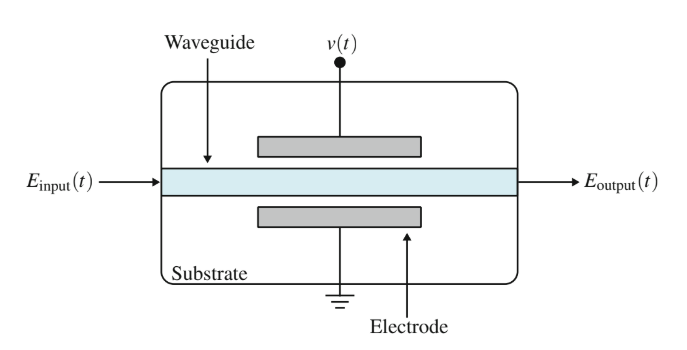
\includegraphics[width=\linewidth]{ModuladorDeFase}
    \caption{Modulador de fase}
  \end{subfigure}
  \hfill
  \begin{subfigure}[b]{0.47\linewidth}
    \centering
    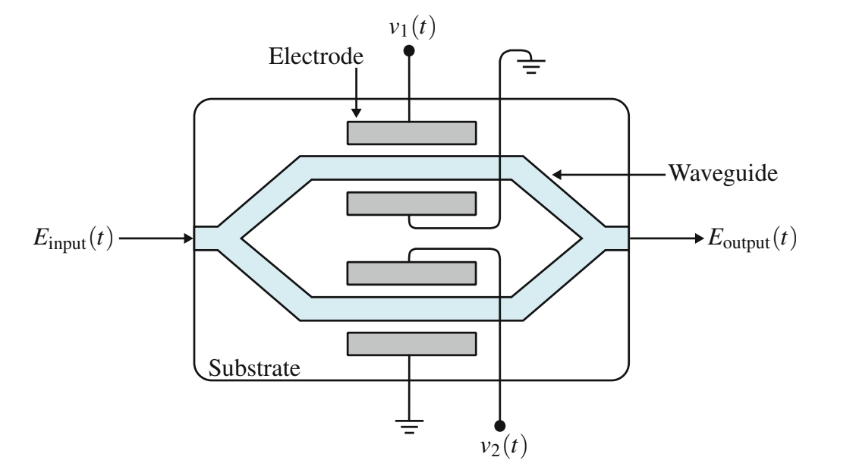
\includegraphics[width=\linewidth]{ModuladorMZM}
    \caption{Mach-Zehnder}
  \end{subfigure}

  \vspace{0.9em}
  \begin{subfigure}[b]{0.52\linewidth}
    \centering
    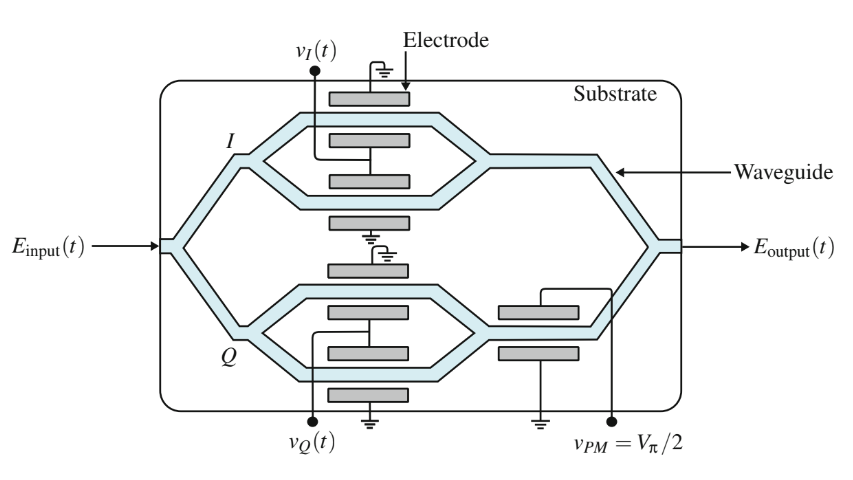
\includegraphics[width=\linewidth]{ModuladorIQ}
    \caption{Modulador IQ}
  \end{subfigure}
  \hfill
  \begin{subfigure}[b]{0.44\linewidth}
    \centering
    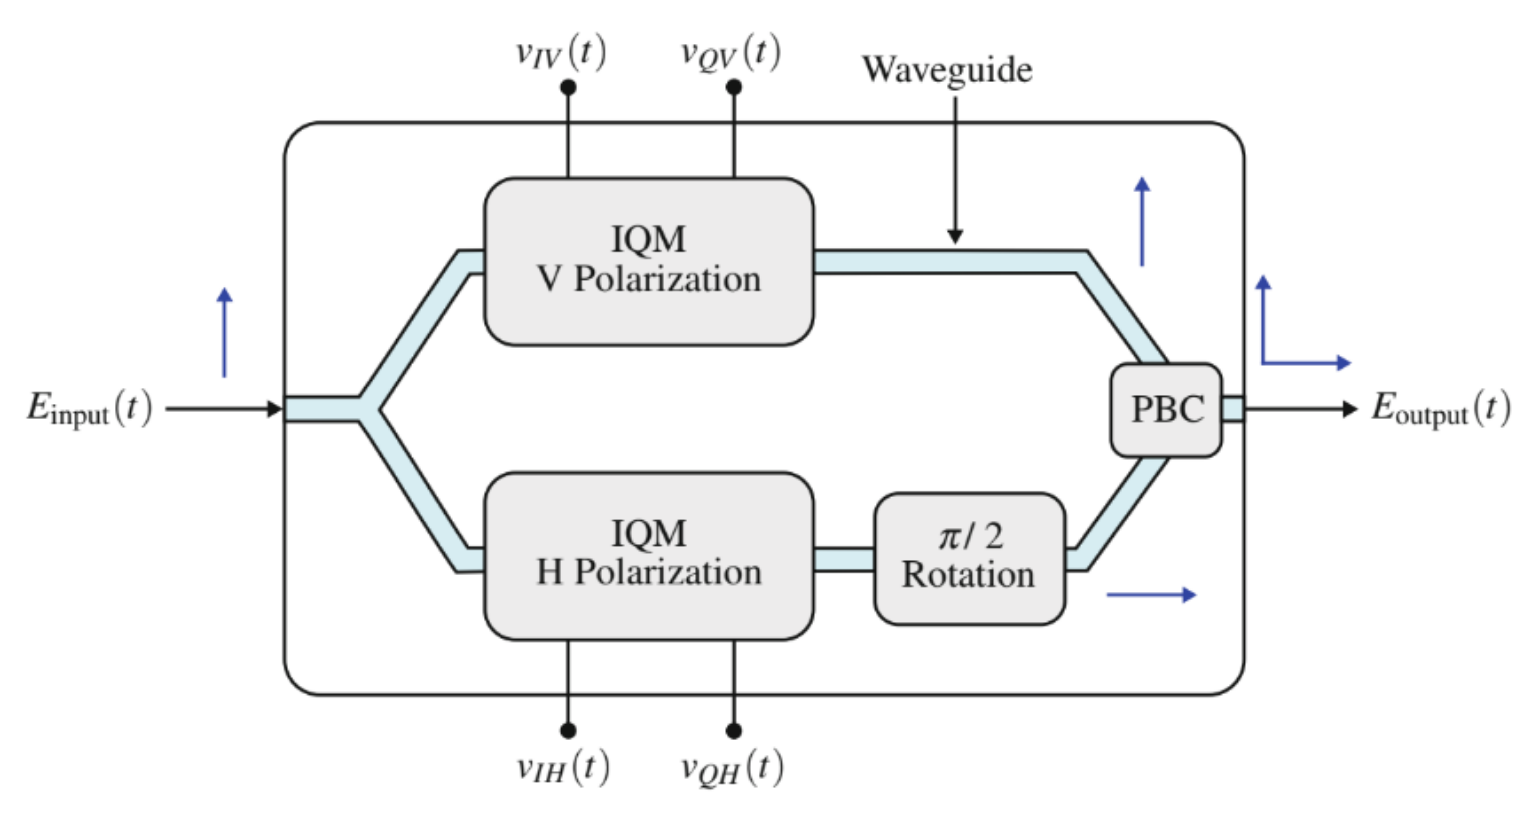
\includegraphics[width=\linewidth]{ModuladorDP}
    \caption{Modulador DP-IQ}
  \end{subfigure}
  \caption[Estructura del modulador DP-IQ]{%
    Estructura anidada del modulador, de adentro hacia afuera. (a)~El
    modulador de fase: un \'unico electrodo sobre una gu\'ia de onda.
    (b)~Dos moduladores de fase en las ramas de un interfer\'ometro forman un
    modulador Mach-Zehnder. (c)~Dos Mach-Zehnder en paralelo, m\'as un
    modulador de fase polarizado en $V_\pi/2$ que introduce el desfasaje de
    $\pi/2$, forman un modulador IQ. (d)~Dos moduladores IQ y un combinador de
    polarizaci\'on (PBC) forman el modulador DP-IQ, con cuatro entradas
    el\'ectricas. Adaptado de~\cite{mello2021}.}
  \label{fig:modulador}
\end{figure}

El componente elemental es el modulador de fase de la \cref{fig:modulador}a.
Este es un electrodo sobre una gu\'ia de onda cuyo \'indice de refracci\'on
depende del campo el\'ectrico aplicado. No cambia la amplitud del campo
entrante, en otras palabras, produce una modulaci\'on de fase proporcional a
la tensi\'on aplicada $v(t)$,
\begin{equation}
  \frac{E_{\mathrm{output}}}{E_{\mathrm{input}}}
     = \exp\!\left(j\,\frac{\pi v}{V_\pi}\right),
  \label{eq:pm}
\end{equation}
donde $E_{\mathrm{input}}$ y $E_{\mathrm{output}}$ son los campos \'opticos a
la entrada y a la salida del dispositivo. La tensi\'on $V_\pi$ es la que
produce un desfasaje de $\pi$ \si{\radian}. En base a esto se construye todo
lo dem\'as.

Poniendo un modulador de fase en cada rama de un interfer\'ometro se obtiene
un modulador Mach-Zehnder, que aparece en la \cref{fig:modulador}b. Si los dos
brazos se manejan con tensiones arbitrarias $v_1$ y $v_2$, la recombinaci\'on
da
\begin{equation}
  \frac{E_{\mathrm{output}}}{E_{\mathrm{input}}}
     = \frac{1}{2}\left[
       \exp\!\left(j\frac{\pi v_1}{V_\pi}\right) +
       \exp\!\left(j\frac{\pi v_2}{V_\pi}\right)\right].
  \label{eq:mzm-general}
\end{equation}

En sistemas de comunicaciones \'opticas coherentes, estos moduladores operan
en lo que se conoce como configuraci\'on push-pull, en la que los dos brazos
se manejan con tensiones id\'enticas y opuestas, $v_1 = -v_2 = v/2$.
Reemplazando en \eqref{eq:mzm-general},
\begin{equation}
  \frac{E_{\mathrm{output}}}{E_{\mathrm{input}}}
     = \frac{1}{2}\left[
       e^{\,j\pi v/2V_\pi} + e^{-j\pi v/2V_\pi}\right]
     = \cos\!\left(\frac{\pi v}{2V_\pi}\right).
  \label{eq:mzm}
\end{equation}

Dos moduladores MZ en paralelo forman un modulador IQ, representado en la
\cref{fig:modulador}c. Cada uno se polariza en el nulo,
$V_{\mathrm{bias}} = -V_\pi$. Una de las dos ramas lleva adem\'as un modulador
de fase fijo en $v_{PM} = V_\pi/2$, que aporta el desfasaje de $\pi/2$ entre
ellas. Llamando $m_I$ y $m_Q$ a las tensiones de modulaci\'on medidas desde el
punto de polarizaci\'on, la salida resulta
\begin{equation}
  \frac{E_{\mathrm{output}}}{E_{\mathrm{input}}}
     = \frac{1}{2}\left[
       \sin\!\left(\frac{\pi m_I}{2V_\pi}\right) +
       j\,\sin\!\left(\frac{\pi m_Q}{2V_\pi}\right)\right],
  \label{eq:iqm}
\end{equation}
donde el seno aparece porque $\cos(\pi(m-V_\pi)/2V_\pi) = \sin(\pi m/2V_\pi)$,
y el factor $1/2$ da cuenta del divisor de entrada y del combinador de salida.
Con \eqref{eq:iqm} se puede obtener la constelaci\'on QPSK a partir de se\~nales
el\'ectricas, $m_I$ y $m_Q$.

Finalmente, el modulador DP-IQ, representado en la \cref{fig:modulador}d, se
construye a partir de dos moduladores IQ y un combinador de polarizaci\'on
(PBC, \emph{polarization beam combiner}). Cada modulador IQ genera una se\~nal
\'optica modulada de manera independiente, a partir de dos se\~nales
el\'ectricas que controlan sus componentes en fase y cuadratura. Las salidas
de ambos moduladores se combinan mediante el PBC en dos polarizaciones
ortogonales. Se obtiene as\'i una se\~nal \'optica con modulaci\'on
independiente en ambas polarizaciones, controlada por las cuatro se\~nales
el\'ectricas $v_{IV}$, $v_{QV}$, $v_{IH}$ y $v_{QH}$.



\subsubsection*{P\'erdidas por modulaci\'on}

Cada Mach-Zehnder se polariza en el nulo de transmisi\'on,
$V_{\mathrm{bias}} = -V_\pi$, que es lo que permite que el campo tome valores
positivos y negativos. La consecuencia es que la se\~nal trabaja sobre la zona
lineal de la ecuaci\'on~\eqref{eq:mzm}, lejos de sus m\'aximos y m\'inimos, lo
que resulta en p\'erdidas de potencia.

\begin{figure}[H]
  \centering
  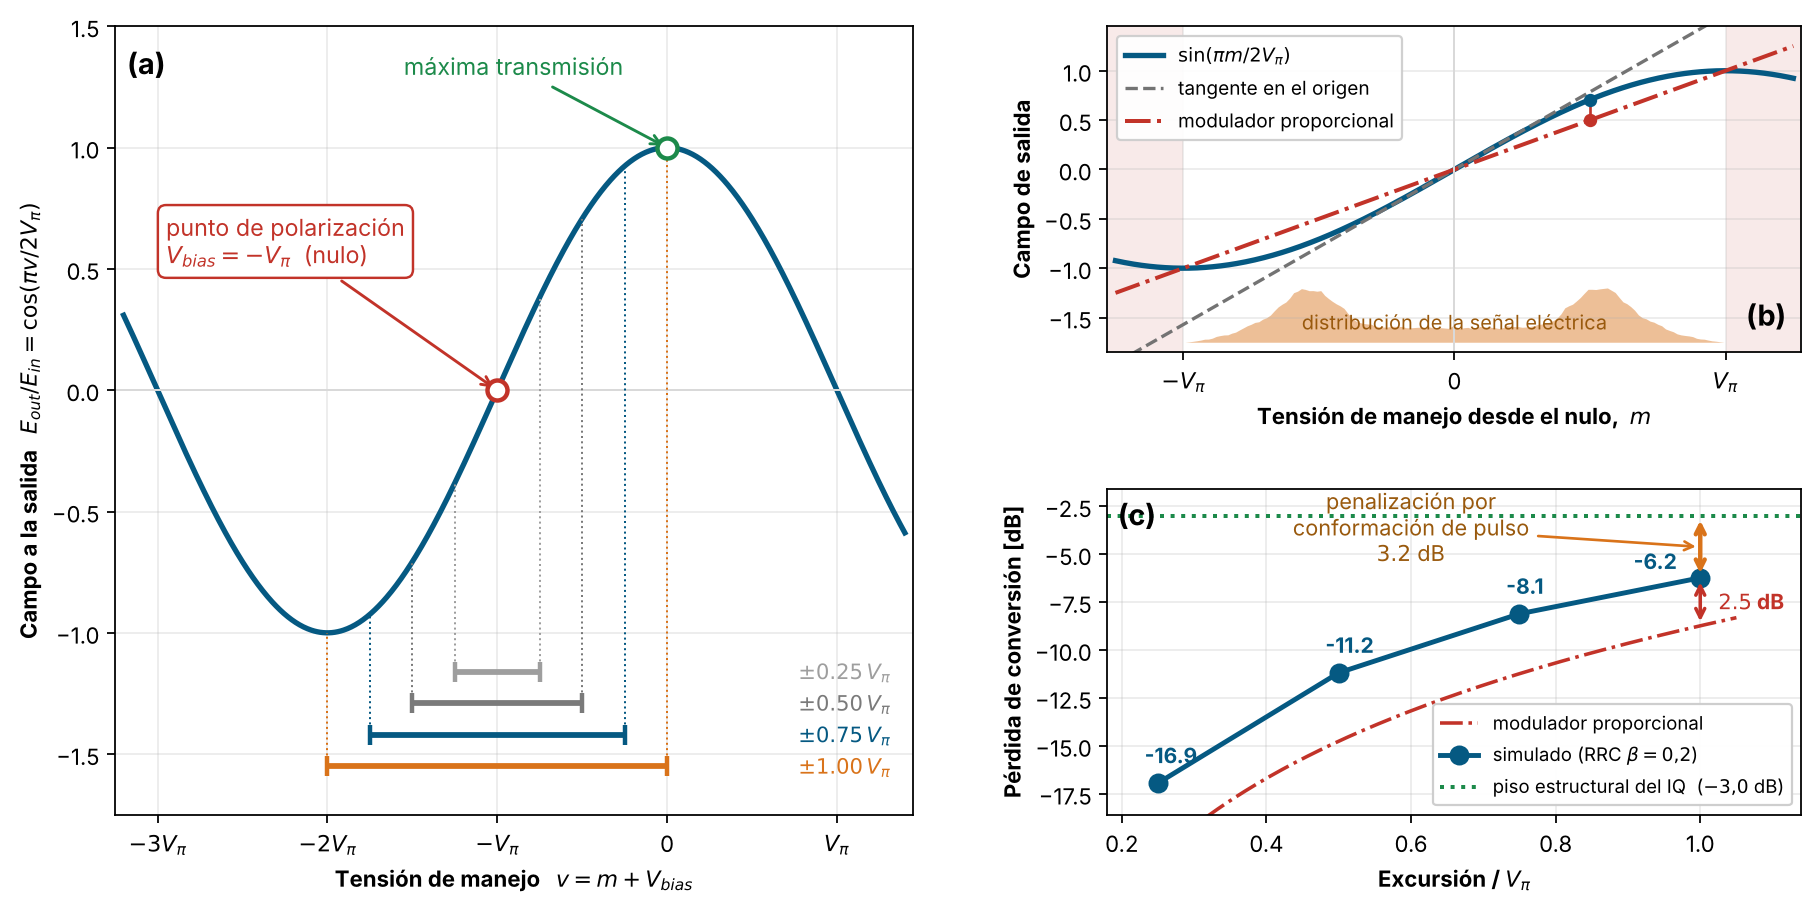
\includegraphics[width=\linewidth]{mzm_punto_polarizacion}
  \caption[Punto de polarizaci\'on y p\'erdida por modulaci\'on del modulador]{%
    Origen de la p\'erdida por modulaci\'on.
    (a)~Polarizado en el nulo, la se\~nal recorre la zona lineal positiva de  $\cos(\pi v/2V_\pi)$. Solo con excursi\'on plena
    $\pm V_\pi$ se llega al m\'aximo del campo.
    (b)~Vista desde el nulo, la transferencia es casi lineal en el centro y se
    comprime cerca de $\pm V_\pi$. Sobre el eje horizontal, la densidad de amplitudes de
    la se\~nal el\'ectrica.
    (c)~P\'erdida contra excursi\'on. La l\'inea punteada es
    el piso de p\'erdida del modulador IQ, \SI{-3.0}{\dB}, que corresponder\'ia
    a se\~nal el\'ectrica binaria. La distancia entre ese piso y el valor simulado
    a excursi\'on plena, \SI{3.2}{\dB}, es la penalidad por conformar el pulso.}
  \label{fig:mzm-bias}
\end{figure}

La \cref{fig:mzm-bias} ilustra el origen de estas p\'erdidas en un modulador
MZ, descomponiendo el efecto en dos contribuciones distintas. La primera es un
piso estructural de \SI{3.01}{\dB}. Si la se\~nal el\'ectrica fuese binaria y
llegara siempre exactamente a $\pm V_\pi$, la ecuaci\'on~\eqref{eq:iqm}
dar\'ia $E_{\mathrm{output}}/E_{\mathrm{input}} = (\pm 1 \pm j)/2$, cuyo
m\'odulo vale $\sqrt{1/2}$. Es decir, un modulador ideal pierde la mitad de
la potencia de entrada. Este es el mejor caso posible de un modulador IQ,
representado por la l\'inea punteada del panel~(c).

La segunda es la penalizaci\'on dependiente de la conformaci\'on del pulso,
que para el \emph{roll-off} adoptado implica \SI{3.2}{\dB} adicionales. Su
origen es el factor de cresta. La se\~nal conformada con RRC pasa la mayor
parte del tiempo lejos de sus picos, con una relaci\'on entre potencia de pico
y potencia media de \SI{5.7}{\dB}. Como la excursi\'on se fija por el
m\'aximo, que no puede superar $V_\pi$, la amplitud media queda muy por debajo
de ese m\'aximo.

La penalizaci\'on, sin embargo, no son \SI{5.7}{\dB} sino \SI{3.2}{\dB}, y la
diferencia la explica la forma de la funci\'on de transferencia. La
\cref{fig:mzm-bias}b compara tres curvas. La primera es la transferencia del
modulador, $\sin(\pi m/2V_\pi)$. La segunda es su tangente en el origen, que
marca el r\'egimen de peque\~na se\~nal. La tercera es la recta que une el
origen con el punto de excursi\'on plena, que es lo que entregar\'ia un
modulador proporcional limitado por el mismo pico. Sobre el eje horizontal se
dibuja adem\'as la densidad de amplitudes de la se\~nal el\'ectrica.

En la \cref{fig:mzm-bias}b, el seno queda por encima de la curva roja en todas las amplitudes
intermedias. A $m = 0{,}5\,V_\pi$ entrega \num{0.71} en lugar de \num{0.50}.
Lo que decide la penalidad, de todos modos, no es un punto aislado sino la
potencia media de salida sobre toda la distribuci\'on de amplitudes.
Promediando sobre la se\~nal conformada, el modulador proporcional entrega
$\langle (m/V_\pi)^2 \rangle = \num{0.266}$ y el modulador real entrega
$\langle \sin^2(\pi m/2V_\pi) \rangle = \num{0.474}$. El cociente entre los
dos son \SI{2.5}{\dB}, que es lo que se recupera de los \SI{5.7}{\dB} del
factor de cresta. La penalidad neta por conformaci\'on resulta entonces de
\SI{3.2}{\dB}.

Sumando las dos contribuciones, la p\'erdida a excursi\'on plena es de
\SI{6.2}{\dB}. Reducir la excursi\'on empeora la p\'erdida r\'apidamente, porque cerca del
nulo la transferencia es casi lineal y la potencia depende entonces del
cuadrado de la se\~nal. Por lo tanto, cada vez que se reduce a la mitad la
excursi\'on se pierden casi \SI{6}{\dB}. A $\pm 0{,}5\,V_\pi$ la p\'erdida es
de \SI{11.2}{\dB} y a $\pm 0{,}25\,V_\pi$ llega a \SI{17.0}{\dB}. Por este
motivo, se decidi\'o como criterio de dise\~no usar un modulador operando a la
m\'axima excursi\'on.

Por \'ultimo, la p\'erdida de \SI{6.2}{\dB} contabiliza \'unicamente la
geometr\'ia de la modulaci\'on, ya que ignora el acoplamiento a fibra, la
propagaci\'on por las gu\'ias de onda, los divisores y el combinador de
polarizaci\'on. Un modulador DP-IQ comercial de niobato de litio para
\SI{32}{\giga\baud} especifica hasta \SI{14}{\dB} de p\'erdida de inserci\'on
total~\cite{fujitsu_ftm7977}. Por este motivo, el balance de potencia del
\cref{cap:enlace} adopta un valor de p\'erdidas de modulaci\'on total de
$L_{\mathrm{DP}} = \SI{14}{\dB}$. El modelo implementado describe bien la
forma de la se\~nal, pero subestima la p\'erdida total del dispositivo.

\section{L\'aser}
\label{sec:trx-laser}

El l\'aser se representa por su campo \'optico complejo, con dos fuentes de
ruido incorporadas al modelo. El ruido de fase se genera como una caminata
aleatoria de incrementos gaussianos con varianza $2\pi\dnu\,T$, que produce el
espectro lorentziano de la \cref{fig:linewidth}. A su vez, el RIN se modela
multiplicando la potencia instant\'anea por un factor aleatorio, de manera que
la fluctuaci\'on de amplitud es siempre una fracci\'on de la potencia.

Escribiendo $P(t) = P_0\,[1 + n(t)]$ con $n$ de media nula, el RIN es la
densidad espectral de esa fluctuaci\'on relativa, y su valor integrado en un
ancho de banda $B$ vale $\sigma_n^2 = \mathrm{RIN}\cdot B$. El campo resulta
\begin{equation}
  E(t) = \sqrt{P_0\,[1+n(t)]}\;e^{\,j\varphi(t)}
       \simeq \sqrt{P_0}\left[1 + \frac{n(t)}{2}\right] e^{\,j\varphi(t)},
  \label{eq:rin-campo}
\end{equation}
donde la aproximaci\'on vale para $|n| \ll 1$ y $\varphi$ es el ruido de fase
descripto arriba. La perturbaci\'on de amplitud tiene entonces potencia
$P_0\,\sigma_n^2/4$, y la relaci\'on se\~nal-ruido que impone el RIN queda
\begin{equation}
  \mathrm{SNR}_{\mathrm{RIN}} = \frac{4}{\mathrm{RIN}\cdot B}.
  \label{eq:snr-rin}
\end{equation}

\begin{figure}[H]
  \centering
  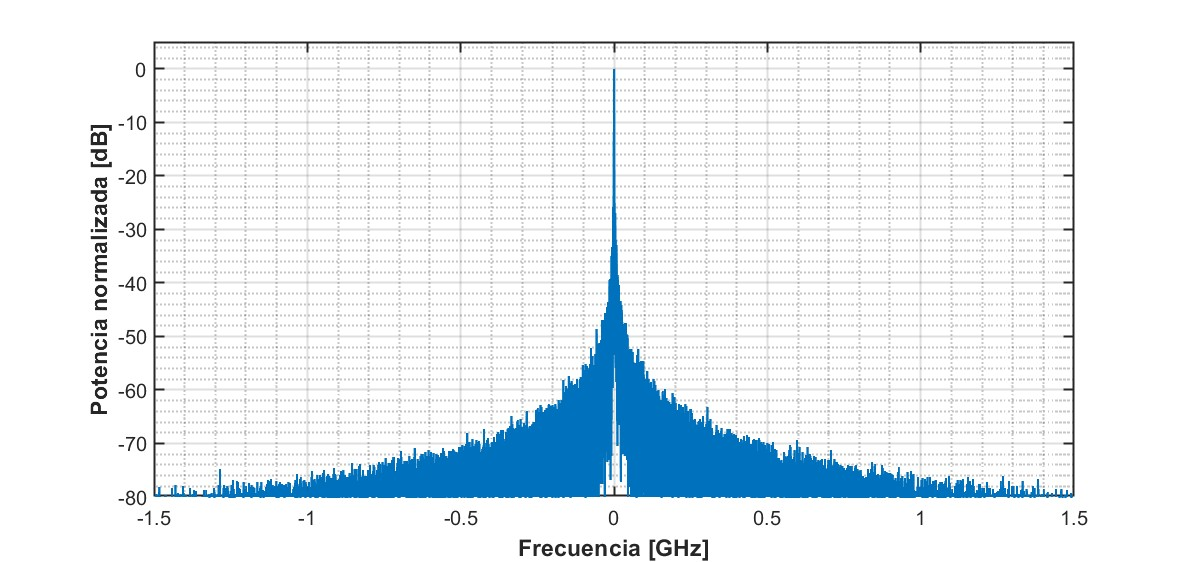
\includegraphics[width=0.72\linewidth]{LineWidth}
  \caption[Espectro del l\'aser simulado]{%
    Espectro de potencia del l\'aser simulado. La forma lorentziana, con las
    colas cayendo como $1/f^2$ alrededor de la portadora, es caracter\'istica del
    ruido de fase modelado como caminata aleatoria.}
  \label{fig:linewidth}
\end{figure}

El l\'aser transmisor y el oscilador local usan el mismo modelo. Sus
par\'ametros se eligieron tomando como referencia un m\'odulo sintonizable
comercial, el PPCL500~\cite{ppcl500}, que cubre toda la banda C con una
potencia de salida de hasta \SI{17}{\dBm}, un ancho de l\'inea 
t\'ipico de \SI{15}{\kilo\hertz} y un RIN de \SI{-140}{\dB\per\hertz}. El RIN
de la simulaci\'on es el correspondiente a la hoja de datos. El ancho de l\'inea, en cambio,
se llev\'o a $\dnu = \SI{100}{\kilo\hertz}$ por l\'aser, un orden de magnitud
por encima del valor real, para exigir al lazo de recuperaci\'on de fase m\'as
de lo que el componente impone.

La tolerancia del receptor a los dos ruidos del l\'aser se analiza en el
\cref{cap:tolerancias}, barriendo cada uno contra una familia de valores de
OSNR.

\section{Front-end coherente y muestreo del receptor}
\label{sec:trx-rx}


El receptor usa una arquitectura de recepci\'on coherente con diversidad de
polarizaci\'on, seg\'un la \cref{fig:receptor}. Un divisor de haz por
polarizaci\'on (PBS) separa las componentes $H$ y $V$ tanto de la se\~nal
recibida como del oscilador local. A su vez, cada par entra a un h\'ibrido de
\SI{90}{\degree} como el descripto en la \cref{sec:coh-deteccion}. Finalmente,
las ocho salidas \'opticas van a parar a cuatro fotodetectores balanceados,
cada uno seguido de su amplificador de transimpedancia y su ADC.

\begin{figure}[H]
  \centering
  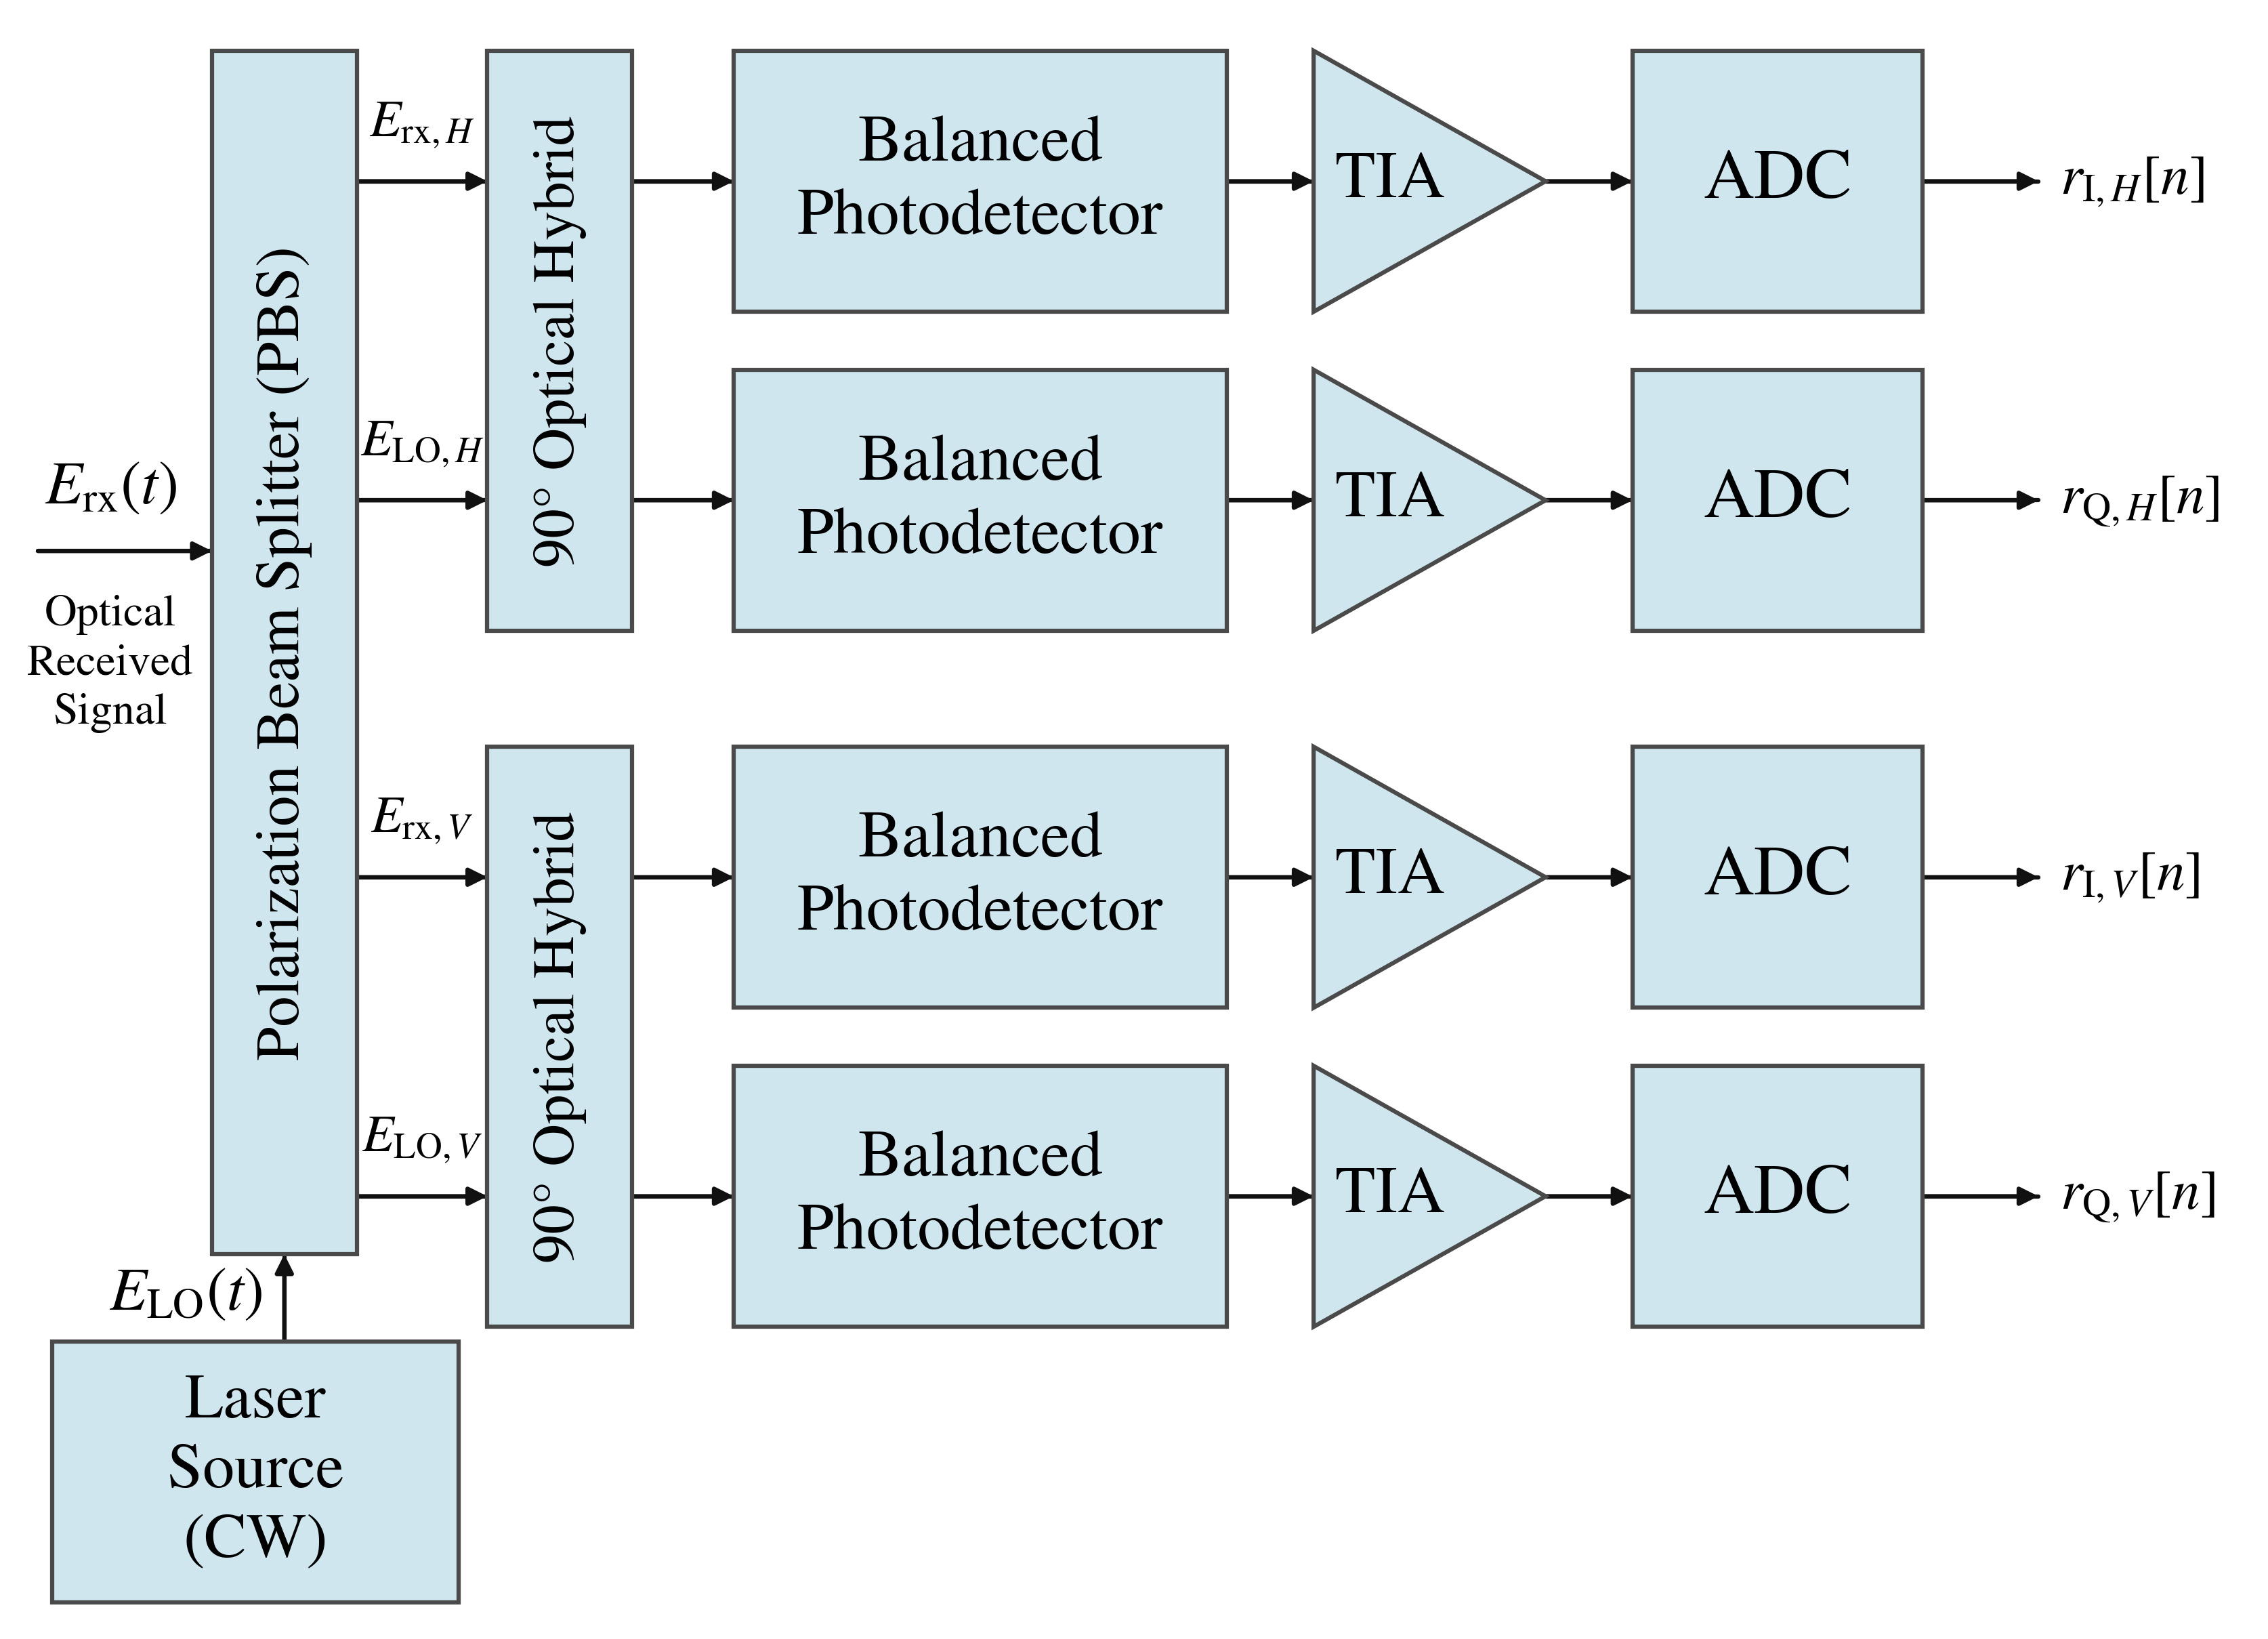
\includegraphics[width=0.72\linewidth]{receptor_esquema}
  \caption[Front end coherente de doble polarizaci\'on]{%
    Front end coherente de doble polarizaci\'on. El mismo oscilador local
    alimenta las dos ramas, de modo que el error de frecuencia y el ruido de
    fase son comunes a las cuatro se\~nales digitalizadas.}
  \label{fig:receptor}
\end{figure}

Como el oscilador local es uno solo para las dos
polarizaciones, el error de frecuencia y el ruido de fase son
comunes a $r_{I,H}$, $r_{Q,H}$, $r_{I,V}$ y $r_{Q,V}$, y eso es lo que permite
estimarlos una \'unica vez sobre las dos polarizaciones en lugar de dos veces
por separado.
\subsection{Respuesta de los fotodiodos, el TIA y el ADC}
\label{sec:trx-anchos}

La respuesta en frecuencia de la cadena de recepci\'on se model\'o con filtros
de Bessel de quinto orden, que aproximan bien la fase lineal de este tipo de
componentes. Se aplican dos, uno por cada limitaci\'on de ancho de banda.

\begin{itemize}\itemsep2pt
  \item El front end \'optico, es decir, los fotodetectores m\'as los
        amplificadores de transimpedancia (TIA), con \SI{20}{\giga\hertz} de
        ancho de banda a \SI{3}{\dB}.
  \item El ADC, con \SI{33}{\giga\hertz} de ancho de banda.
\end{itemize}

Los dos valores se tomaron de las hojas de datos del equipamiento contra el
que despu\'es se contrasta la simulaci\'on en el \cref{cap:experimental}.

\begin{figure}[H]
  \centering
  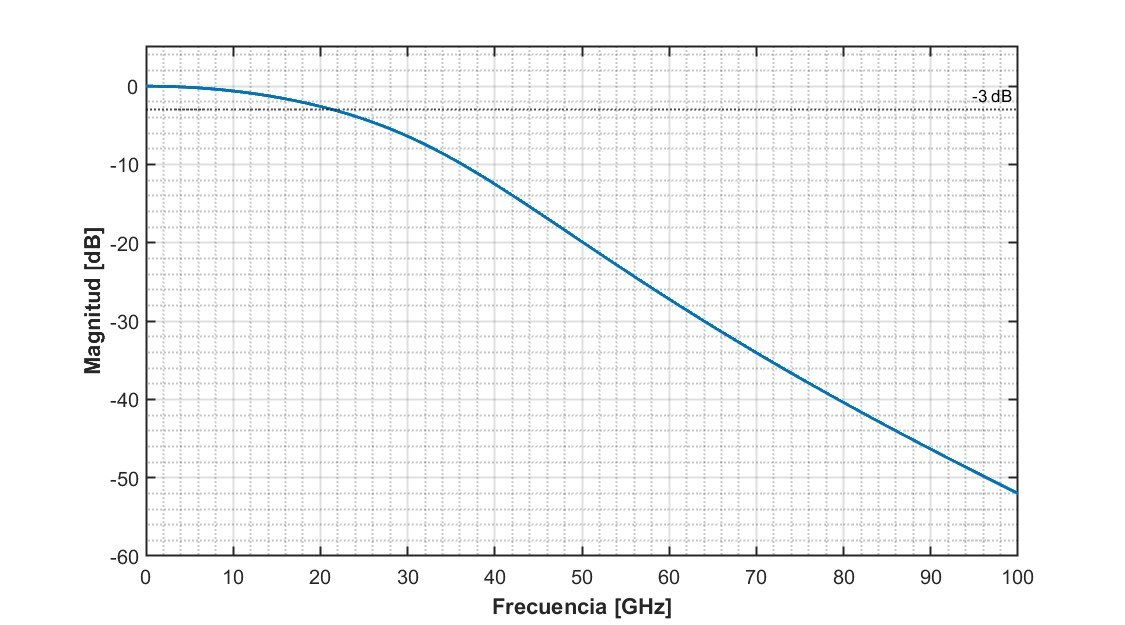
\includegraphics[width=0.70\linewidth]{FiltroTIA_Bessel5toOrden}
  \caption[Respuesta del filtro del TIA]{%
    Respuesta en magnitud del front end, modelado como
    Bessel de quinto orden con el punto de \SI{-3}{\dB} en
    \SI{20}{\giga\hertz}. Los \SI{19.2}{\giga\hertz} que ocupa la se\~nal
    quedan dentro del ancho de banda de \SI{3}{\dB}.}
  \label{fig:filtro-tia}
\end{figure}

La \cref{fig:filtro-tia} muestra la respuesta del front end. Conviene recordar
que la se\~nal ocupa un ancho de banda en banda base de \SI{19.2}{\giga\hertz},
seg\'un la ecuaci\'on~\eqref{eq:ancho-senal}. Este valor cae justo antes del
punto de \SI{-3}{\dB}, de modo que el front end es, de los dos bloques, el que
m\'as recorta el espectro de la se\~nal.

\begin{figure}[H]
  \centering
  \begin{tikzpicture}[
    font=\footnotesize, >={Latex[length=2mm]},
    bl/.style ={draw, rounded corners=3pt, align=center,
                minimum height=3.6em, text width=9.0em, inner sep=3pt},
    cl/.style ={draw=red!40, rounded corners=3pt, fill=red!8, align=center,
                minimum height=3.2em, text width=11.0em, inner sep=3pt},
    fl/.style ={->, thick}
  ]
    \node[bl] (f) {Filtro de Bessel\\[1pt]de quinto orden\\[1pt]
                   $B_{\mathrm{ADC}}=\SI{33}{\giga\hertz}$};
    \node[bl, right=3.0em of f] (s) {Muestreo\\[1pt]$16 \to 2$ muestras\\[1pt]
                   por s\'imbolo};
    \node[cl, below=2.4em of s] (c) {Error de reloj\\[1pt]
                   $t_k = k\,\Ts(1+\delta) + \tau_0$};

    \draw[fl] ($(f.west)-(3.0em,0)$)
      node[left, align=right, font=\scriptsize] {16 muestras\\ por s\'imbolo}
      -- (f.west);
    \draw[fl] (f) -- (s);
    \draw[fl] (c) -- (s);
    \draw[fl] (s.east) -- ++(3.0em,0)
      node[right, align=left, font=\scriptsize] {2 muestras\\ por s\'imbolo};
  \end{tikzpicture}
  \caption[Modelo del ADC]{%
    Modelo del ADC. El filtro de Bessel reproduce la respuesta anal\'ogica de
    la etapa de entrada del conversor. El muestreo posterior lleva la se\~nal a las dos
    muestras por s\'imbolo con las que trabaja el DSP, con
    los instantes afectados por el error de frecuencia de muestreo $\delta$ y
    por el desfasaje inicial $\tau_0$.}
  \label{fig:adc}
\end{figure}

El ADC se representa mediante un modelo simplificado de dos etapas, como
muestra la \cref{fig:adc}. La primera reproduce la respuesta en frecuencia de
la etapa anal\'ogica de entrada del conversor, mediante el filtro pasabajos
de Bessel de quinto orden con ancho de banda de \SI{3}{\dB} de
\SI{33}{\giga\hertz}. La segunda modela el proceso de muestreo, con una
reducci\'on de la tasa de la simulaci\'on de \num{16} a \num{2} muestras por
s\'imbolo, que es la tasa a la que opera el receptor digital. Sobre esta
segunda etapa act\'ua el error de reloj, de modo que los instantes de muestreo
resultan $t_k = k\,\Ts(1+\delta) + \tau_0$, con $\delta$ el error de
frecuencia de muestreo de la \cref{sec:canal-doppler} y $\tau_0$ el desfasaje
inicial.

En cuanto a la conversi\'on de amplitud, se considera un ADC ideal de
resoluci\'on infinita. No se incorpora cuantizaci\'on y las muestras se
mantienen en formato de punto flotante.


\subsection{Elecci\'on de la tasa de muestreo}
\label{sec:trx-nyquist}

El ancho de banda anal\'ogico de un ADC suele quedar por debajo de la mitad de
su frecuencia de muestreo, de modo que la propia etapa de entrada act\'ua como
filtro anti-aliasing. En este caso, el ancho de banda es fijo e igual a \SI{33}{\giga\hertz},
mientras que la frecuencia de muestreo depende de la tasa de s\'imbolo,
$f_s = \mathrm{SpS}\cdot\Rs$. Como este trabajo opera a distintas tasas, la
frecuencia de muestreo cambia con ellas y hace falta verificar que en ning\'un
caso aparezca solapamiento. Lo que decide esa condici\'on es el ancho de banda
de la se\~nal $B$ y no el del conversor.

Se decidi\'o utilizar una tasa de dos muestras por s\'imbolo. Muestrear replica el
espectro cada $f_s$, de modo que la condici\'on de no solapamiento entre
r\'eplicas es $f_s \geq 2B$, es decir
\begin{equation}
  \mathrm{SpS} \geq 1 + \beta = 1{,}2 .
  \label{eq:sps-min}
\end{equation}

\begin{figure}[H]
  \centering
  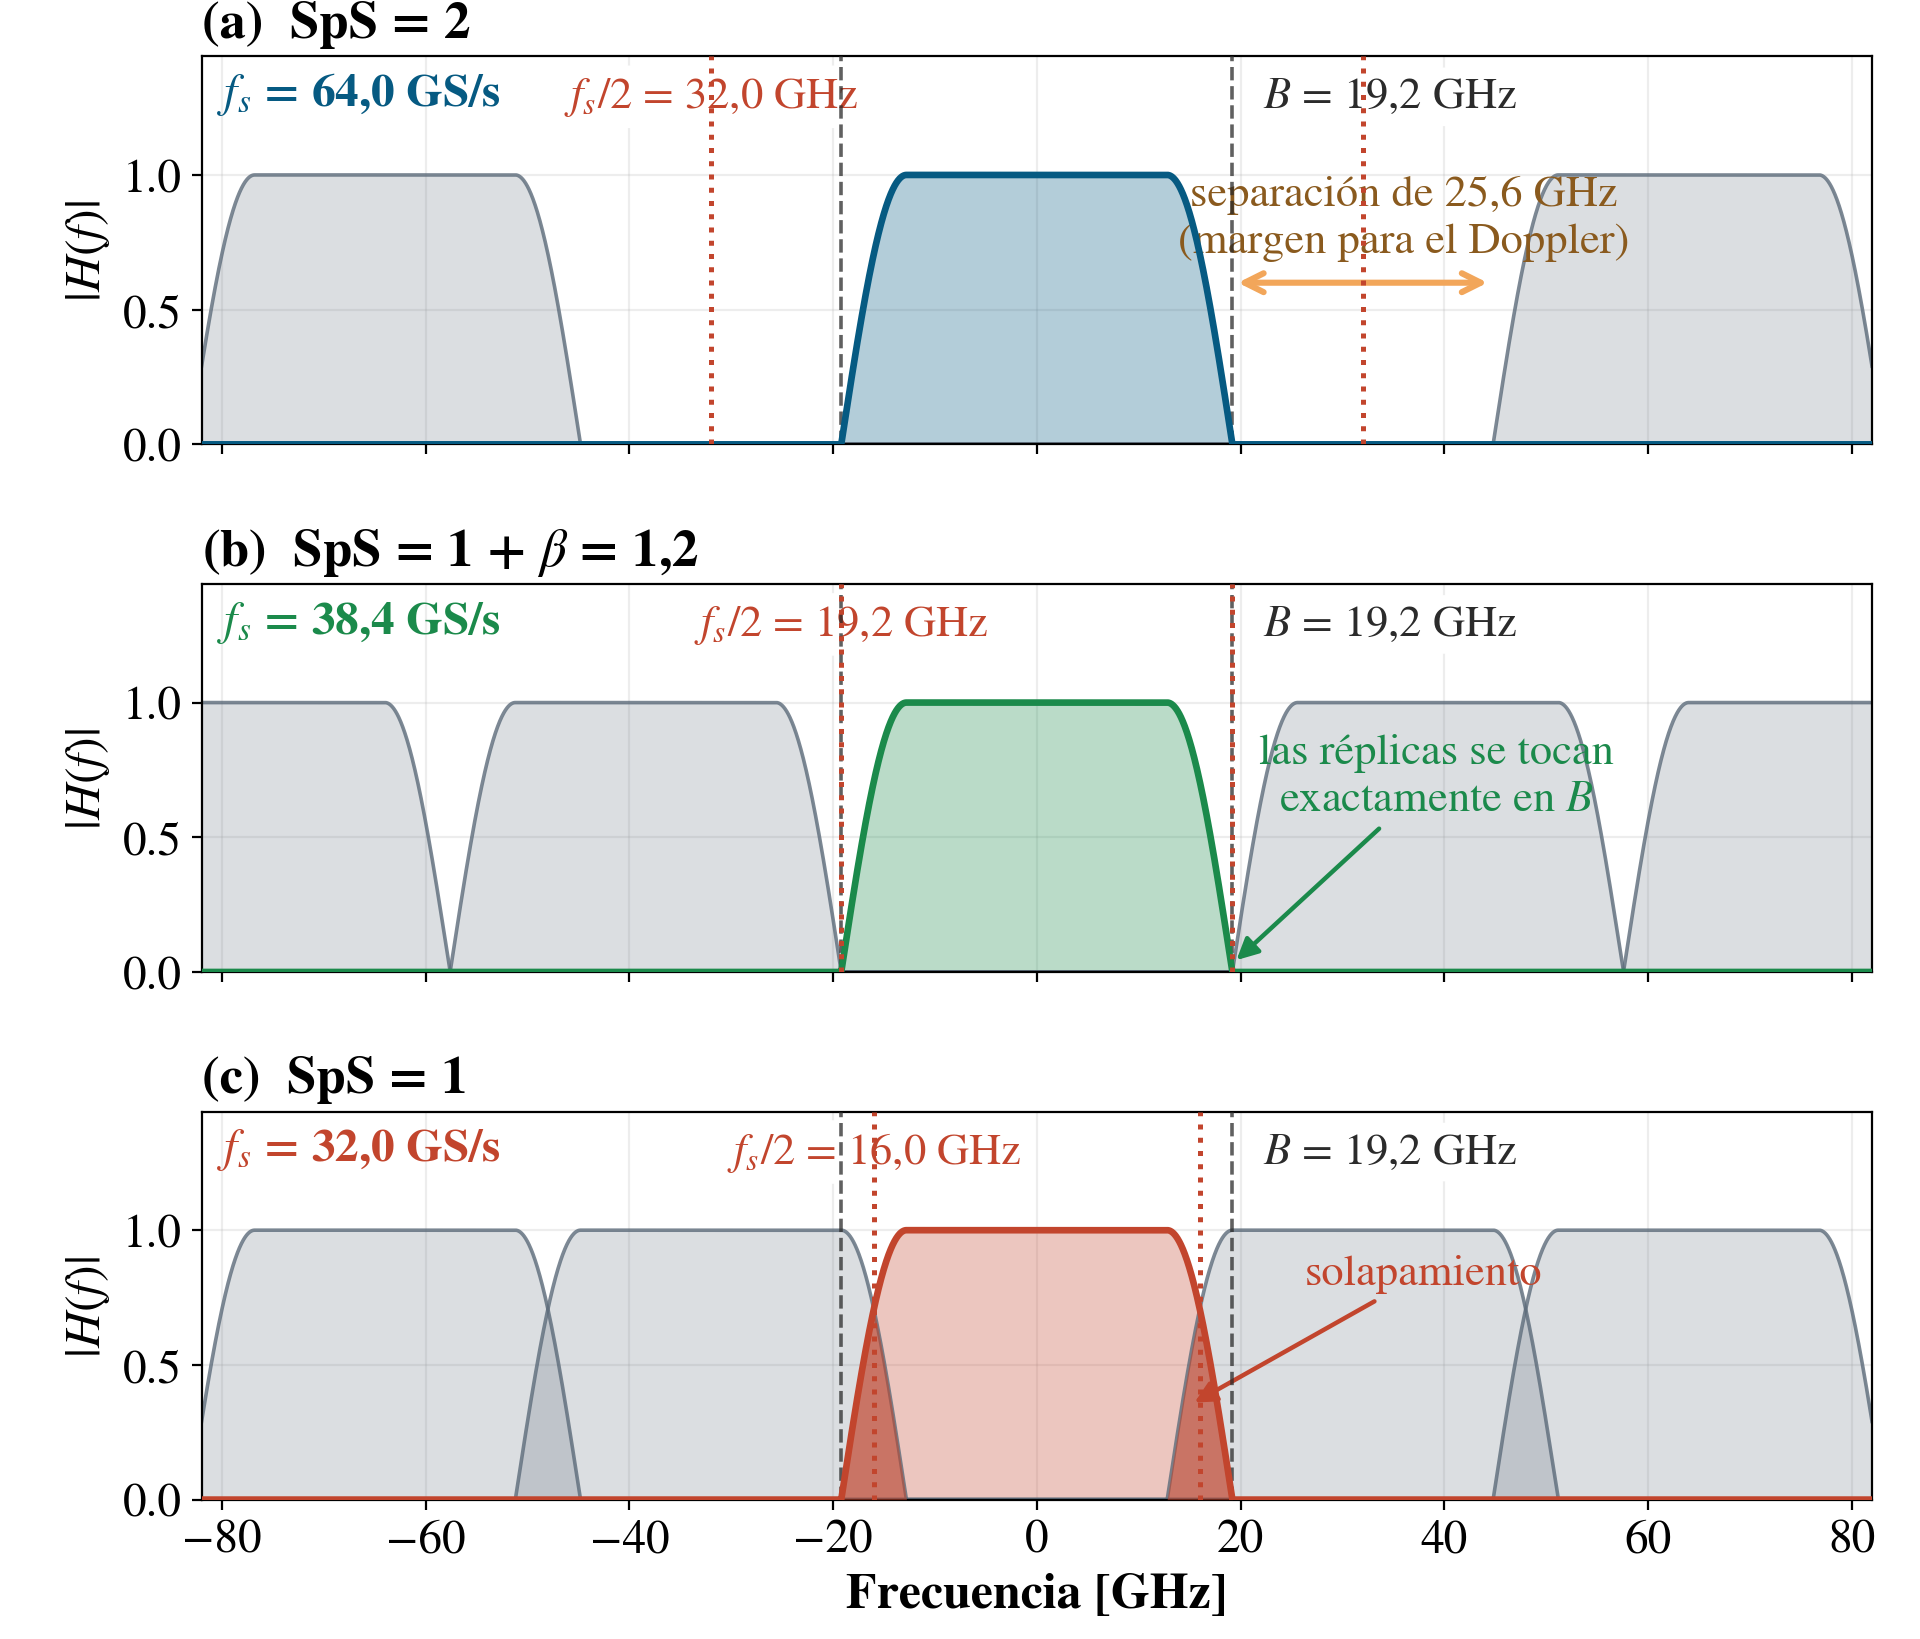
\includegraphics[width=0.88\linewidth]{nyquist_sps}
  \caption[Elecci\'on de la tasa de muestreo]{%
    Espectro muestreado para tres tasas. Con $\mathrm{SpS} = 2$ queda una
    separaci\'on de \SI{25.6}{\giga\hertz} entre la se\~nal y su r\'eplica. Con
    el m\'inimo te\'orico $\mathrm{SpS} = 1{,}2$ las r\'eplicas se tocan
    exactamente en $B$, y con $\mathrm{SpS} = 1$ se superponen y hay aliasing
    irreversible.}
  \label{fig:nyquist}
\end{figure}

La \cref{fig:nyquist} compara las tres situaciones. El m\'inimo te\'orico,
$\mathrm{SpS} = 1{,}2$, deja las r\'eplicas toc\'andose exactamente en $B$, de
modo que cumple Nyquist pero sin ning\'un margen. Con $\mathrm{SpS} = 2$, en
cambio, $f_s = \SI{64}{\giga\hertz}$ y queda una separaci\'on de
\SI{25.6}{\giga\hertz} entre la se\~nal y su r\'eplica.

Este margen es el que absorbe el desplazamiento Doppler. La se\~nal llega
centrada en $\Df$ y ocupa $[\Df - B,\ \Df + B]$, de manera que para que no se
pliegue al muestrear tiene que entrar por completo en la banda,
$\pm f_s/2$. La condici\'on resulta
\begin{equation}
  \abs{\Df} \;\leq\; \frac{f_s}{2} - B
            \;=\; \frac{\Rs\left[\mathrm{SpS} - (1+\beta)\right]}{2},
  \label{eq:doppler-alias}
\end{equation}
que con dos muestras por s\'imbolo se reduce a $\Rs(1-\beta)/2 =
\SI{12.8}{\giga\hertz}$. El requisito de captura del enlace es de
\SI{6.0}{\giga\hertz}, as\'i que el muestreo no es un problema. El verdadero limitante es el recuperador de frecuencia del DSP, cuyo
rango de captura se mide en el \cref{cap:tolerancias}.


\section{Desbalances considerados}
\label{sec:trx-noideal}

Sobre la cadena ideal se inyectan cuatro deterioros que no provienen del canal
sino del equipamiento, resumidos en la \cref{tab:noideal}.

\begin{table}[htbp]
\centering

\begin{tabular}{llc}
\toprule
\textbf{Deterioro} & \textbf{Origen} & \textbf{Valor} \\
\midrule
Desbalance IQ    & h\'ibrido de \SI{90}{\degree}     & \SI{10}{\degree} \\
Skew I/Q         & largo el\'ectrico de los carriles & \SIrange{-1.0}{1.5}{\pico\second} \\
Error de reloj   & Doppler (canal)                   & \SI{25.55}{\ppm}\\
                 & oscilador del Rx (hardware)       & \SI{5}{\ppm} \\
Fase de muestreo & instante de muestreo del ADC      & $0{,}25\,\Ts$\\
\bottomrule
\end{tabular}
\caption[No idealidades inyectadas y su origen f\'isico]{No idealidades inyectadas y su origen f\'isico. El error de reloj
suma dos contribuciones de naturaleza distinta: el Doppler del canal y la
deriva del oscilador local del receptor.}
\label{tab:noideal}
\end{table}

El desbalance IQ es la desviaci\'on de la cuadratura del h\'ibrido, por la cual
las dos salidas no son completamente ortogonales. Un receptor
coherente presenta t\'ipicamente entre \SIrange{1}{5}{\degree}. Se adopt\'o \SI{10}{\degree} para la validaci\'on del DSP.

El skew surge debido a la diferencia entre los caminos el\'ectricos que recorren las ramas I y Q de cada polarizaci\'on. Esta diferencia se acumula en todo el trayecto, desde el híbrido hasta los cables que entran al ADC. A \SI{32}{\giga\baud} un símbolo dura \SI{31.25}{\pico\second}, de modo que \SI{1.5}{\pico\second} son \num{0.048} tiempos de símbolo.

El error de reloj tiene dos or\'igenes distintos. Uno es el Doppler de reloj de la
ecuaci\'on~\eqref{eq:dop-sfo}, \SI{25.55}{\ppm}, que es una propiedad del
canal. Y el otro hace referencia al error de frecuencia de muestreo del ADC del receptor, unos
\SI{5}{\ppm}, que es una propiedad del equipo. Los dos se manifiestan como el
mismo error de frecuencia de muestreo y se inyectan sumados, aunque su origen
sea distinto. A esto se agrega un offset fijo del instante de muestreo, de
$0{,}25\,\Ts$, que representa la falta de sincronismo entre el reloj del
digitalizador y el del transmisor.

\section{Conclusiones}
\label{sec:trx-conclusiones}


En este cap\'itulo se desarroll\'o un modelo general del transmisor y del
receptor, desde la generaci\'on de s\'imbolos hasta el muestreo con error de
reloj y de fase. Los par\'ametros se eligieron despu\'es, tomando como
referencia los dispositivos del laboratorio, lo que permite contrastar
simulaci\'on y medici\'on en el \cref{cap:experimental}.


El modulador opera a excursi\'on plena,
porque reducirla empeora la p\'erdida de modulaci\'on con rapidez. El roll-off
$\beta = 0{,}2$ mantiene la se\~nal dentro del ancho de banda del front end sin privar al detector
de reloj del exceso de ancho de banda que necesita. Las dos muestras por
s\'imbolo dejan lugar para que el offset Doppler desplace la se\~nal dentro de
la banda digitalizada.

El conversor no cuantiza, de modo
que sus \'unicos efectos sobre la se\~nal son el filtrado y el submuestreo. Y el
modelo del modulador contabiliza solo la geometr\'ia de la modulaci\'on, por
lo que subestima la p\'erdida del dispositivo real. El balance de potencia del
\cref{cap:enlace} adopta en su lugar $L_{\mathrm{DP}} = \SI{14}{\dB}$, tomado
de un componente comercial.

Este modelo se utilizado para el resto del trabajo. Los algoritmos que recuperan la
se\~nal se describen en el \cref{cap:dsp}, el balance de potencia en el
\cref{cap:enlace} y los l\'imites de tolerancia de cada deterioro, incluidos
los dos ruidos del l\'aser, en el \cref{cap:tolerancias}.